\newpage
\chapter{Grundverständnis}
In diesem Kapitel befassen wir uns mit den ersten paar Aufgaben und wollen ein Grundlagenverständnis des Computers und
seiner Funktionsweise aufbauen, welches wir später verwenden, um allfällige Probleme oder Verhaltensweisen besser
verstehen zu können. Hierbei stellt sich also die Frage, wie so ein Gerät aufgebaut ist und wie die einzelnen Komponenten zusammenspielen, die
wir hauptsächlich verwenden. Wir zeigen hier euch auch, was euch z.B. in einer Berufsschule erwarten könnte oder sogar erwarten wird. Ihr
seht, womit ihr euch unter vielem anderen auseinandersetzen werdet.\\\\
\textbf{Was du in diesem Kapitel sehen wirst:}\\
$\square$ Was ist die CPU und wofür ist sie zuständig?\\
$\square$ Wie kann der Computer mit Zahlen arbeiten?\\
$\square$ Wie können zwei Zahlen addiert werden?\\
$\square$ Was ist eine logische Operation?\\
$\square$ Was ist die RAM und wofür ist sie zuständig?\\
$\square$ Wie kann ich mir etwas im Computer merken oder speichern?

\newpage
\section{Der Leader}
Die \gls{CPU} bildet das Herzstück eines Computers. Sie ist zuständig, um verschiedene Instruktionen auszuführen. Wenn
z.B. zwei Zahlen addiert werden sollen, dann ist die CPU das Stück Hardware, welches diese Arbeit erledigt.\par
\begin{minipage}{\linewidth}
    \centering
    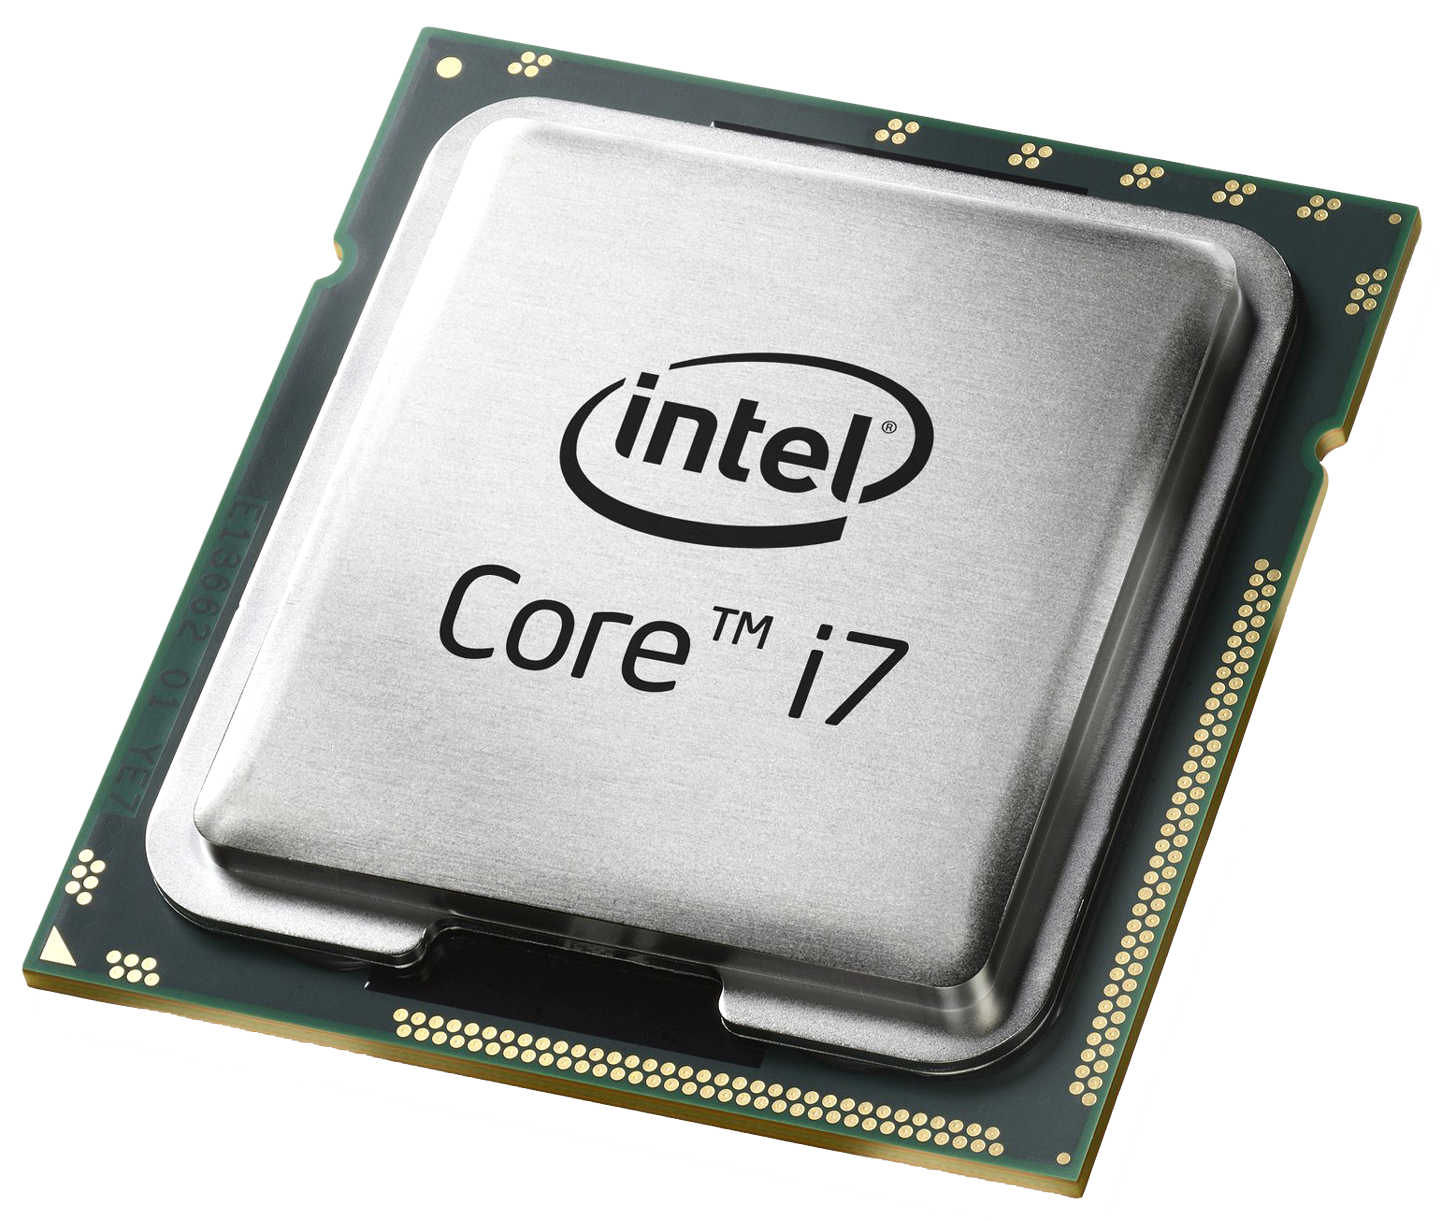
\includegraphics[width=0.2\textwidth]{../common/chapter_02/resources/01_cpu_intel.png}
    \captionof{figure}{Intel CPU}
\end{minipage}
Nun fragt man sich zurecht, wie die CPU denn solche Aufgaben bewältigen kann? Dazu muss man wissen, dass die CPU
selbst wiederum aus mehreren Teilen besteht, die alle eine bestimmte Aufgabe erfüllen. Es sind dies im Wesentlichen:
\begin{description}
    \item[Control unit] Diese Einheit steuert den ganzen Ablauf der CPU. Sie sagt den anderen Komponenten im Gerät und
    in der CPU selbst, was sie wann tun sollen und steuert so den ganzen Computer.\cite{wikipedia:cu}
    \item[Arithmetic logic unit] Wenn arithmetische oder logische Operationen durchgeführt werden sollen, dann ist diese
    Einheit wichtig. Wenn z.B. 4 + 5 gerechnet werden soll, dann wird die ALU damit beauftragt.\cite{wikipedia:alu}
    \item[Address generation unit] Will die CPU auf den Hauptspeicher (RAM) zugreifen, dann wird in dieser Einheit die korrekte
    Adresse berechnet. Was das genau bedeutet wird im nächsten Abschnitt erklärt.\cite{wikipedia:agu}
\end{description}
Die CPU beinhaltet noch mehr solcher Einheiten, auf diese wird aber nun nicht mehr weiter eingegangen.
\subsection{Übung 1 - Computer und Zahlen}
Es wird Zeit für die erste kleine Übung. Wir wollen darin das Verständnis stärken, wie Zahlen überhaupt in einem Computer
dargestellt werden und wie wir in der Lage sind, diese zu addieren.\\
Du hast sicher schon gehört, dass ein Computer mit 1en und 0en arbeitet. Wir wollen uns nun anschauen, was das genau bedeutet.\\
Dazu musst du dir aber erst mal darüber klar werden, wie wir Menschen uns Zahlen vorstellen, respektive, wie wie wir
sie darstellen.\\
Nehmen wir als Beispiel die Zahl $145$.
Natürlicherweise, wissen wir sofort, wie viel das ist, wir machen uns aber nicht
wirklich über den Aufbau an sich Gedanken. Wir wollen nun diese Zahl ein wenig anders formulieren.\\
Wir finden darin eine 1, diese steht ganz links an dritter Stelle. Sie bildet die Wertigkeit 100. Die zweite Ziffer ist eine
4, sie steht in der Mitte an zweiter Stelle und bildet die Wertigkeit 10. Die dritte Ziffer steht ganz rechts an erster Stelle
und bildet die Wertigkeit 1.\\\\
Ausgangslage dieser Zahl ist nun erstmal die 1.\\
Die Frage stellt sich jetzt, wie wir die 1 an die Stelle ganz links verschieben können.
Wir haben dazu das Werkzeug der Multiplikation und können z.B. die 1 einfach mit der Wertigkeit 100 multiplizieren. Damit
verschieben wir diese an die gewünschte Position.\\
$1 \times 100 = 100$\\
\begin{exerciseseries}[columns=1,solsubrule=\hrule]{}
    \begin{exercise}
        Überlege dir kurz, wie wir die 4 an die Position in der Mitte verschieben können:\\
        $4 \times $\underline{\hspace{1cm}} $ = 40$
    \end{exercise}
    \begin{solution}
        $4 \times 10 = 40$
    \end{solution}

    \begin{exercise}
        Und nun überlege dir, was wir mit der 5 ganz rechts machen müssen?\\
        $5 \times $\underline{\hspace{1cm}} $ = 5$
    \end{exercise}
    \begin{solution}
        $5 \times 1 = 5$
    \end{solution}
\end{exerciseseries}

\begin{alignat*}{3}
    1 \times && 100 = && 100\\
    4 \times &&  10 = &&  40\\
    5 \times &&   1 = &&   5
\end{alignat*}

\newpage
\subsection{\solutionsname}
\loadSolutions